\documentclass{article}
\usepackage[utf8]{inputenc}
\usepackage{graphicx}
\usepackage{hyperref}
\graphicspath{ {./images/} }


\title{Turn Based Game on Blockchain}
\author{Arora, Harsh MCS2022 \\
        Chakraborty, Arghyadip MCS202206 \\
        Gangamreddypalli, Namratha Reddy MCS202105 \\
        Gantait, Arunava MCS202201 \\
        Iyer, Paarth MCS202218}
\date{December 2022}

\begin{document}

\maketitle
\newpage
\tableofcontents
\newpage

\section{Problem Statement}
The aim of this project is to implement a simple turn-based game on the blockchain.
The particular game implemented is \textbf{Antakshari}, which is played   as follows:
\begin{itemize}
    \item The first player submits a word
    \item At each subsequent turn, player submit a word which begins with the last letter of the previous word.
\end{itemize}
The validity of each submitted word must be checked in some way, e.g. by making calls
to a dictionary maintained by some trusted source outside the blockchain. \textit{Timing constraints} and \textit{elimination criteria} may also be introduced. Passing on a turn may be allowed.



Finally, the game should have some consistent termination and winning criteria.
\section{Main Idea}

% 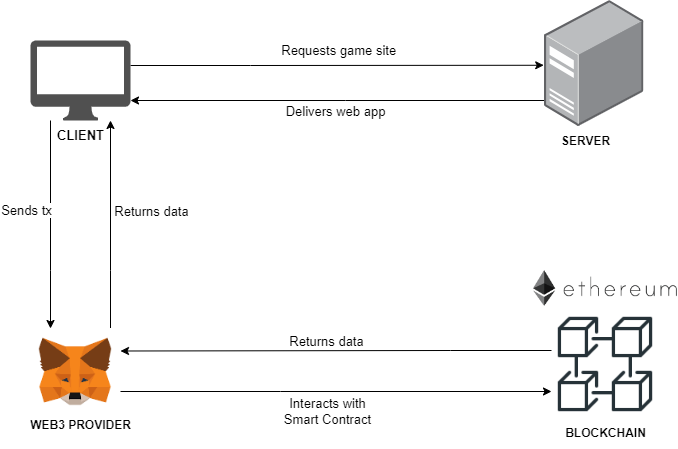
\includegraphics[scale=0.5]{images/arch.png}

\begin{figure}[htp]
    \centering
    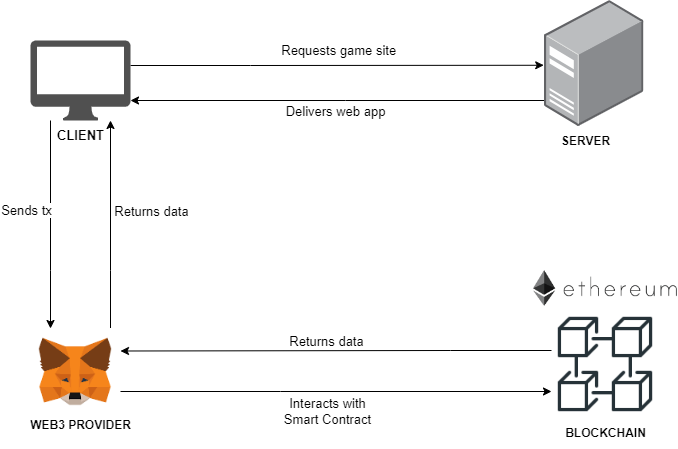
\includegraphics[scale=0.5]{images/arch.png}
    \caption{Architecture diagram}
    % \label{fig:galaxy}
\end{figure}

The client accesses the game website by entering the url in their browser with the Metamask extension. 
After which they play the game by using our frontend and sending transactions via Metamask, which interacts with the Ethereum blockchain, and hence our smart contracts deployed on it.

\paragraph{Key Components}
\begin{itemize}
\item[] \textbf{Ethereum}: It is a decentralized, open-source blockchain with smart contract functionality. Ether is the native cryptocurrency of the platform.
\item[] \textbf{Smart Contract}: They are the building blocks we use to create blockchain applications. They are programs that we can write with source code and deploy to the blockchain. They are written in the Solidity programming language. 
\item[] \textbf{MetaMask}: It serves as a web3 provider and a crypto wallet, whose purpose is to interact with the blockchain. It is distributed as a browser extension. 
\item[] \textbf{Ethers js}: It is a popular library that basically encodes and decodes any data prior to, or after interaction with the blockchain.
% We are using Ethers which is a Web3 JS library.

\end{itemize}



\section{Implementation}

\subsection{Game features}

\begin{itemize}
    \item[] \textbf{Judge}:
    There is a predecided judge who is responsible for approving (validating) each
    submitted word in the game
    \item[] \textbf{Validation Condition}:
    Apart from the condition mentioned in the problem, a word is deemed valid by the
    judge if it has not been used previously (thus we do not allow repitition of words)
    and also if it comes from the dictionary implemented in \verb|worddict.js|
    \item[] \textbf{Lives}:
    We have implemented a system of lives. The issuer of the game contract (the \textit{creator}) gets 3 lives, and any new player gets 5. A life is lost upon
    submission of an invalid word. Losing all lives results in elimination
    \item[] \textbf{Terminating/winning condition}: 
    Our terminating condition is through \textbf{last man standing}. When all but one
    player have been eliminated through the process described above, the remaining
    player is declared the winner.
\end{itemize}

    \subsection{Development tools} 
    \href{https://trufflesuite.com/}{\textit{The Truffle Suite}}:
    Truffle advertises itself as "the most comprehensive suite of tools for smart
    contract development". 
    \paragraph{How it can be used}:
    Truffle can be used as a development environment, testing framework and asset
    pipeline for blockchains using the \emph{Ethereum Virtual Machine} (\textbf{EVM}).
    It manages the entire workflow efficiently for any blockchain-based development.
    Its key features include:
    \begin{itemize}
        \item Built-in smart contract compilation, linking, deployment and binary management.
        \item Deployments and transactions through MetaMask to protect our mnemonic.
        \item External script runner that executes scripts within a Truffle environment.
    \end{itemize}
    \paragraph{How we use it}:
    Our backend is Truffle-based. We have used it for testing our software without having to use the actual Ethereum blockchain and spending actual gas on it.
    
    \href{https://trufflesuite.com/ganache/}{\textit{Ganache}}:
    Ganache is a tool for producing "One-click blockchains". It is a personal blockchain for developing software for Ethereum or even Corda. 
    \paragraph{How it can be used}:
    Using Ganache enables:
    \begin{itemize}
        \item \verb|console.log| in Solidity
        \item Forking any Ethereum network without waiting to sync
        \item Ethereum JSON/RPC support
        \item Impersonating any account without requiring any actual private keys
        \item Listening for JSON-RPC 2.0 requests over HTTPS/WebSockets
        \item Mining blocks instantly, on demand, or at an interval.
    \end{itemize}
    among other things.
    
    \paragraph{How we use it}:
    Ganache has also been used for testing, by simulating players using fake private keys and addresses and observing how our code interacts with requests and events.
    
    %\end{enumerate}



\subsection{Backend}

1. Contract files
2. 

\subsection{Frontend}





\section {Challenges/Improvements}
Could not include a timer because you have to keep track of transaction hashrate:
essentially the only way to know time is when a new block is added to the blockchain. For an auction this is fine since any transaction after the time limit can be discarded. However for our game we want to ensure that every player has a time limit after which the turn proceeds to the next player and every player needs to know which player failed to answer within the time limit. 

Could not include a Merkle tree due to lack of time which would have gotten rid of the judge. Instead we have used another contract (the judge).

\end{document}
